% This is LLNCS.DEM the demonstration file of
% the LaTeX macro package from Springer-Verlag
% for Lecture Notes in Computer Science,
% version 2.4 for LaTeX2e as of 16. April 2010
%
\documentclass{llncs}
%
\usepackage{makeidx}  % allows for indexgeneration
\usepackage{graphicx}
\usepackage{epstopdf}
%
\begin{document}
%

\mainmatter              % start of the contributions
%
\title{An Approach for the Chinese Question-answer System based on Document}
%
\titlerunning{Chinese Question-answer System}  % abbreviated title (for running head)
%                                     also used for the TOC unless
%                                     \toctitle is used
%
\author{Benyou Wang\inst{1} \and Jiabing Niu\inst{1} \and Liqun Ma\inst{1} \and Lipeng Zhang\inst{1} \and Yuhua Zhang\inst{1}
\and Peng Zhang\inst{1}}
%
\authorrunning{Benyou Wang et al.} % abbreviated author list (for running head)
%
%%%% list of authors for the TOC (use if author list has to be modified)
\tocauthor{Benyou Wang, Jiabing Niu, Liqun Ma, Lipeng Zhang, Yuhua Zhang
, and Peng Zhang}
%
\institute{%
Tianjin Key Laboratory of Cognitive Computing and Application, School of Computer Science and Technology, Tianjin University, Tianjin, China\\
% \and Computing and Communications Department, The Open University, United Kingdom \\
% \and Department of Information Engineering, University of Padua, Italy
}



\maketitle              % typeset the title of the contribution

\begin{abstract}
Question Answering system has gradually become a new trend within the field of information retrieval and NLP.It outperforms the conventional search engines,for the system is able to answer users’ questions automatically and accurately.Question Answering system based on English corpus has developed rapidly, whereas the Chinese corpus based Question Answering system still has some problems remains to be solved. Thus, developing a new Question Answering model,which is characterized by dealing with features of Chinese corpus is extemely essentail.Different to the current deep learning model,our model uses the semantic and syntactic information in Chinese corpus and bases on the linearity of Chinese texts.Finally,our model turns out to perform better than other methods through experiments.\dots
\keywords{Question Answer, graph theory, Hamilton cycles}
\end{abstract}
%
\section{Introduction}
%


\section{}
just test a cite\cite{severyn2015learning}

\section{Methods}

\subsection{Data Exploration}

\subsection{Data Exploration}

\subsubsection{Word Overlap and Character Overlap}
It is considered that the more keywords in questions are matched with those in the answer sentences, the more likely that the answer is the correct one.We have found that there are some relationships between the overlapped characters or words and the occurrence frequency of the correct answer after analysing the given corpus.

%\includegraphics[width=3in]{sensitive_simple_trec2013.pdf}

\begin{figure}[htb]
\vspace{2.5cm}
\centering
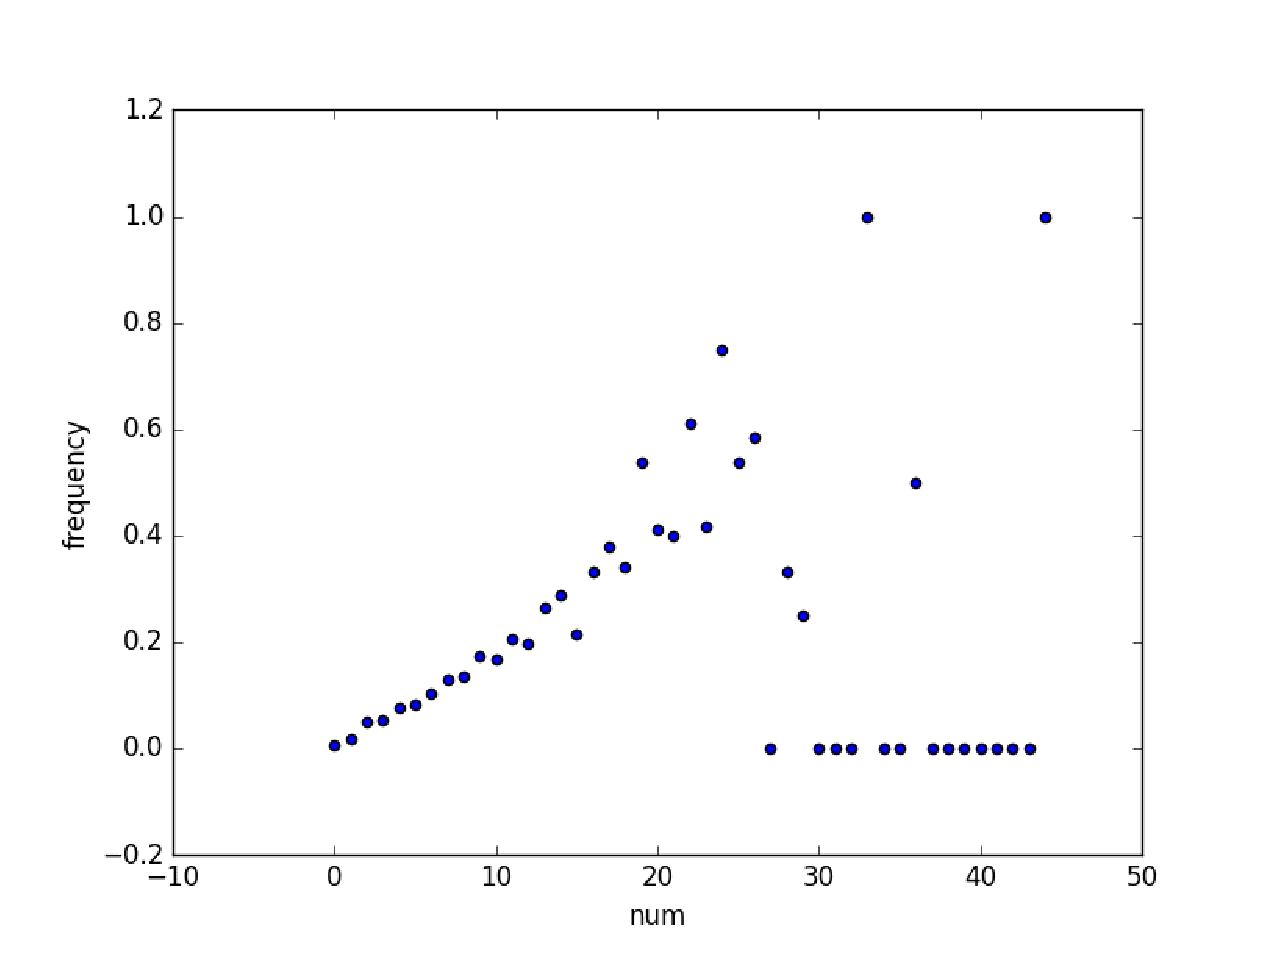
\includegraphics[width=5in]{figures/character_overlap.eps}
\caption{This is the caption of the figure displaying a white eagle and
a white horse on a snow field}
\label{fig:word_character}
\end{figure}



\begin{figure}
\vspace{2.5cm}
\centering
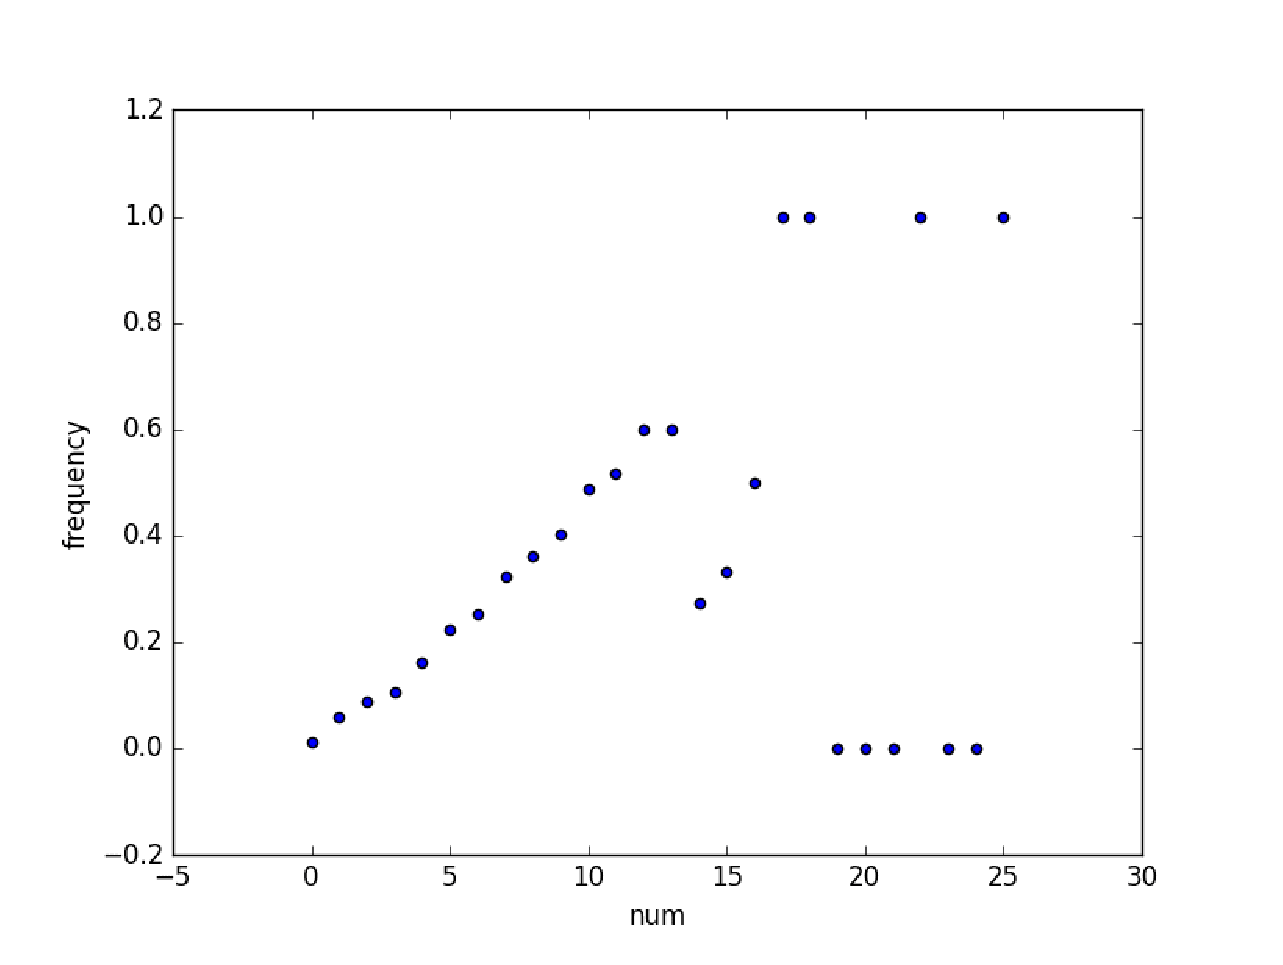
\includegraphics[width=5in]{figures/word_overlap.eps}
\caption{This is the caption of the figure displaying a white eagle and
a white horse on a snow field}
\label{fig:word_overlap}
\end{figure}



\subsubsection{Position Message in Overlapped Words}

\subsubsection{Word Overlap and Character Overlap}

\subsection{Data Preprocessing}

\subsection{Feature Extraction}
\subsubsection{Questions and Answers’ Type}
\subsubsection{Overlap}
\subsubsection{Other Conventional Methods}
\subsubsection{Embedding}

\subsection{Model Selection}

\section{Experimental results}




\section{Discussion and Conclution}



%
% ---- Bibliography ----
%
% \begin{thebibliography}{}
%
% \bibitem{Rodriguez.{2010}}
% Open Source Cloud Computing Tools: A Case Study with a Weather Application
% Rodriguez-Martinez, M.; Seguel, J.; Greer, M.
% Cloud Computing (CLOUD), 2010 IEEE 3rd International Conference on
% Year: 2010
\bibliography{nlpcc_qa}
% \bibliographystyle{IEEEtran}

% \end{thebibliography}



\clearpage
\addtocmark[2]{Author Index} % additional numbered TOC entry
\renewcommand{\indexname}{Author Index}
\printindex
\clearpage
\addtocmark[2]{Subject Index} % additional numbered TOC entry
\markboth{Subject Index}{Subject Index}
\renewcommand{\indexname}{Subject Index}
\input{subjidx.ind}
\end{document}
